\documentclass{beamer}
\usetheme{Madrid}
\usecolortheme{beaver}
\usepackage{graphicx}
\graphicspath{ {/home/nithin/Pictures/Screenshots} }

%Information to be included in the title page:
\title{Maths Bootcamp}
\author{Anonymous}
\institute{Overleaf}
\date{\today}

\begin{document}

\frame{\titlepage}

\section{Geometry} 
\begin{frame}
    \frametitle{Parallel Lines}

\end{frame}

\subsection{}
\section{Congruent Triangles}
\section{Similarity }
\subtitle{Algebra}
\subtitle{Probability}

\begin{frame}{Definition of Percentage}
    \begin{itemize}
        \item A \textbf{percentage} is a way of expressing a number as a fraction of 100.
        \item It is denoted by the symbol 
        \item The formula to calculate a percentage is:
        $$
        \text{Percentage} = \left( \frac{\text{Part}}{\text{Whole}} \right) \times 100
        $$
        \item Example: If you score 45 out of 60 on a test, the percentage is:
      $$  
        \left( \frac{45}{60} \right) \times 100 = 75\%
       $$
    \end{itemize}
\end{frame}

\begin{frame}
    \frametitle{Ratio vs Rate}
    \begin{figure}[h]    
        \begin{minipage}[b]{0.5\textwidth}
        \centering
        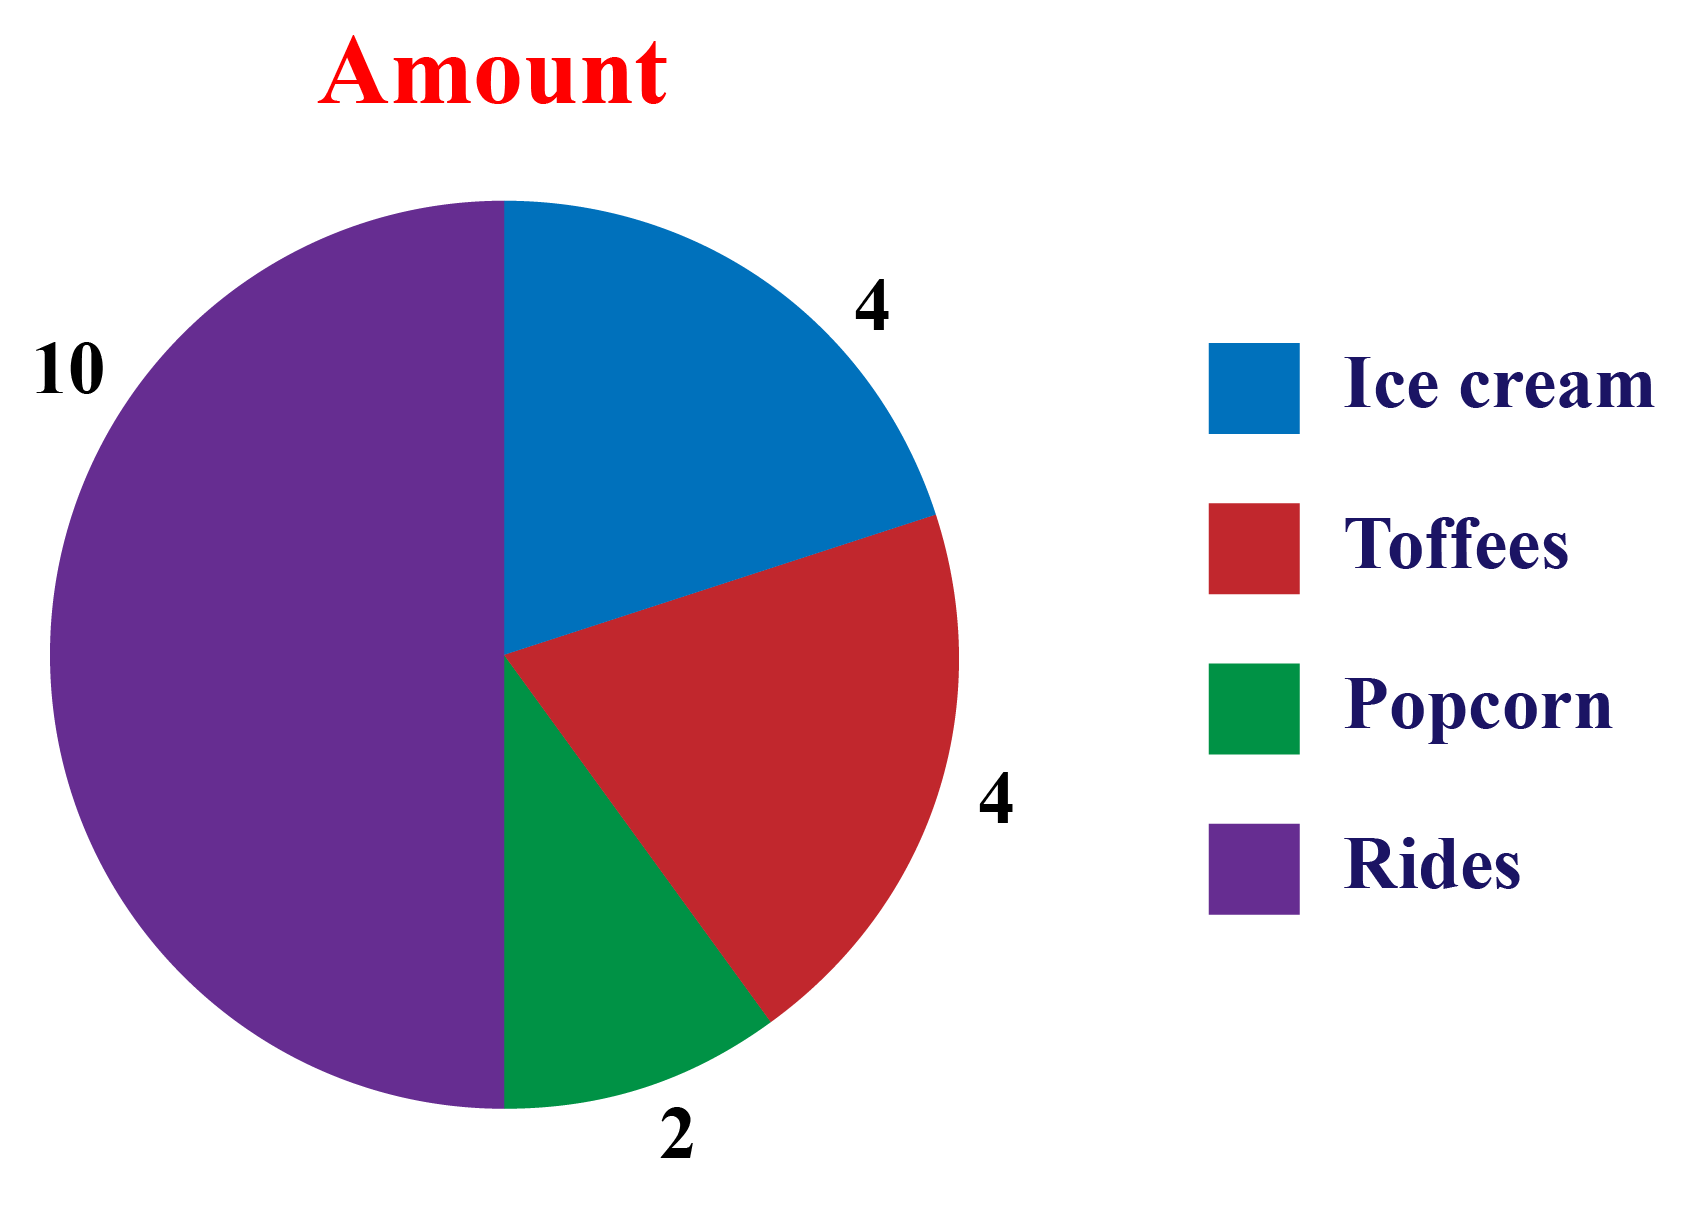
\includegraphics[scale=0.2]{ratio.png}
        \caption{ratio}
    \end{minipage}
    \begin{minipage}[b]{0.4\textwidth}
        \centering
        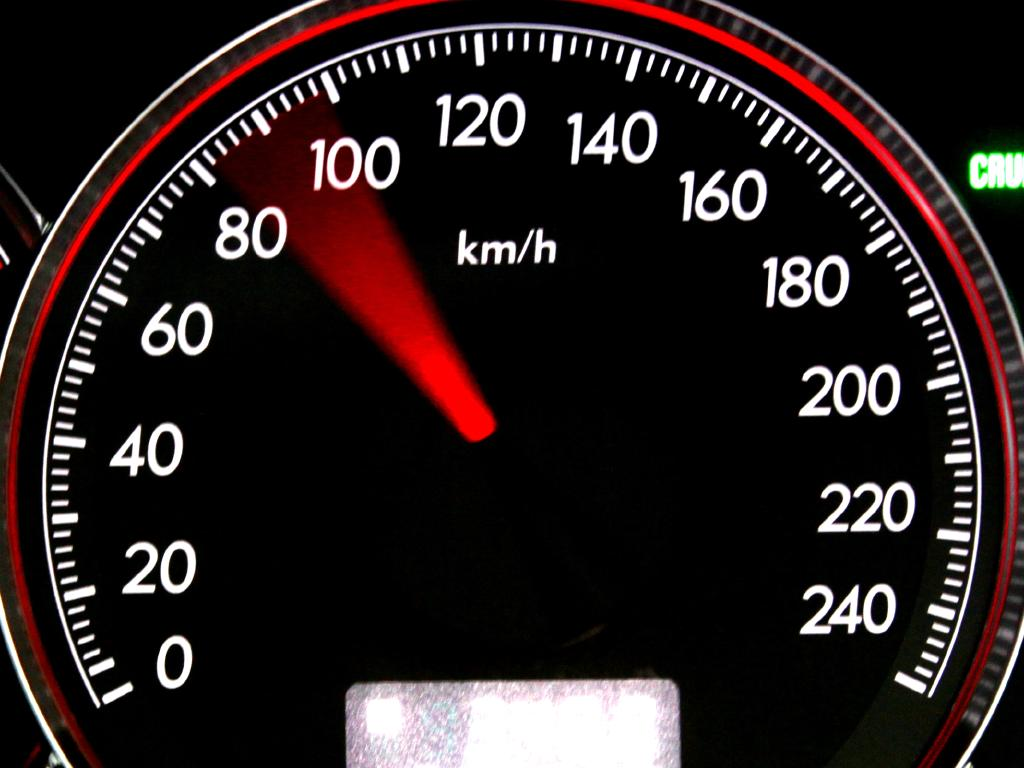
\includegraphics[scale=0.5]{rate.jpeg}
        \caption{rate}
    \end{minipage}
\end{figure}
\end{frame}

    \begin{frame}
    \begin{itemize}
        \item Ratio
            \begin{itemize}
                \item Compares similar quantities
                \item Uses colon notation (e.g., 3:2)
                \item Example: 5 apples to 3 oranges
            \end{itemize}
        \item Rate
            \begin{itemize}
                \item Compares quantities with different units
                \item Expresses change between quantities
                \item Uses "per unit" (e.g., 5 miles per hour)
                \item Example: Cost per pound, heartbeats per minute
            \end{itemize}
    \end{itemize}
\end{frame}

\begin{frame}
    \frametitle{Proportional Relationship}

    \begin{block}{Definition}
        A proportional relationship is a relationship between two quantities where the ratio between them remains constant. 
        If two variables are proportional, it means they can be expressed in the form:
        $$ y = kx $$
        where $ k $ is the constant of proportionality and it can be an integer or a fraction or an irrational number.
    \end{block}
\end{frame}

\begin{frame}
    \frametitle{Proportionality Problem: Mixing Chemicals}

    \begin{block}{Problem}
        A person mixes $15 ml$ of bleach with $3.75 L$ of water for sanitizing solution for a daycare. What are the possible combinations 
    \end{block}

    \begin{itemize}
        \item \textbf{A.} 12 mL bleach and 3L water
        \item \textbf{B.} 6 mL bleach and 1.5L water
        \item \textbf{C.} 3 mL leach and 0.75L water
        \item \textbf{D.} 20 mL bleach and 5.5L water
    \end{itemize}
    \begin{block}{Problem}
        Is the area of square is propotional to side length ?
    \end{block}
\end{frame}

\begin{frame}{Proportionality vs. Linearity}
    \begin{itemize}
        \item A \textbf{proportional relationship} always passes through the origin \((0, 0)\).
        \item The general form of a proportional relationship is:
        \[
        y = kx
        \]
        where \(k\) is the constant of proportionality.
        
        \item A \textbf{linear relationship} can pass through any point, not necessarily the origin.
        \item The general form of a linear relationship is:
        \[
        y = mx + b
        \]
        where \(m\) is the slope and \(b\) is the y-intercept.
        
        \item Key Difference:
        \begin{itemize}
            \item In a proportional relationship, \(b = 0\), so the line always passes through \((0, 0)\).
            \item In a linear relationship, \(b\) can be any value, so the line does not need to pass through the origin.
        \end{itemize}
    \end{itemize}
\end{frame}


\subsection{Statistics}
\begin{frame}
    \frametitle{Variability}
    \begin{block}{Variability}
        Variability refers to how data points differ from one another within a data set. In real-world data, there is almost always some variation because no two measurements, observations, or events are exactly the same.
    \end{block}
\end{frame}

\begin{frame}
    \frametitle{Variability Problems}
        \begin{itemize}
            \item How much does my pet weight ?
            \item What is the average number of cars in a parking lot on Monday mornings ?
            \item Am i hungry?
            \item How often am I hungry after lunch ? 
            \item How much time do you spend on facebook every month? 
        \end{itemize}
\end{frame}
\section{ Geometry}

\begin{frame}
    \frametitle{Eucledian Gemotery}
\end{frame}
\begin{frame}
    \frametitle{Angles}
\end{frame}

\begin{frame}
    \frametitle{Supplementary and Complementary Angles}
       
    \begin{center}
        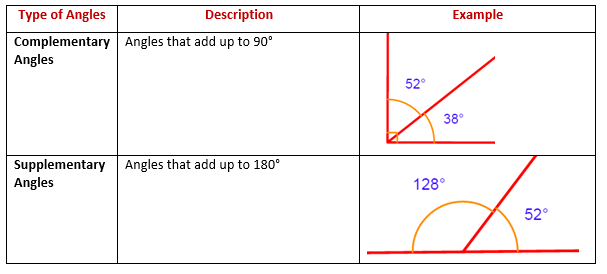
\includegraphics[width=0.9\textwidth]{complementary_supplementary_angles.png} % Add an appropriate image to illustrate supplementary and complementary angles
    \end{center}

\end{frame}

\begin{frame}
    \frametitle{Problem 1}
    
    \begin{center}
        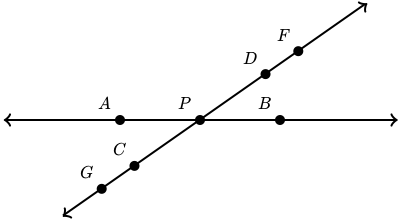
\includegraphics[width=0.9\textwidth]{supplementary_angles.png} % Add an appropriate image to illustrate supplementary and complementary angles
    \end{center}

\end{frame}


\begin{frame}
    \frametitle{Similarity in Triangles}
\end{frame}



\begin{frame}
    \frametitle{Proportional Relationship}
    A relationship between two quantities is proportional if the ratio between those quantities is always equivalent. We will look at side length ratios to find out whether triangles are similar or not
\end{frame}

\begin{frame}{Similarity in All Shapes}
  The concept of similarity applies to any two shapes that have the same \textbf{shape} but may differ in \textbf{size}.
    \vspace{10pt}
    \textbf{Conditions for Similarity}:
    \begin{itemize}
        \item \textbf{Corresponding angles must be equal}: The angles in one shape must match the angles in the other.
        \item \textbf{Corresponding sides must be proportional}: The lengths of corresponding sides must have the same ratio (scaling factor).
    \end{itemize}
\end{frame}

\begin{frame}
    \vspace{10pt}
    \textbf{Examples of Similar Shapes}:
    \begin{itemize}
        \item \textbf{Quadrilaterals}: Squares, rectangles, rhombuses, and parallelograms can be similar if corresponding angles are equal and side lengths are proportional.
        \item \textbf{Polygons}: Any polygons (pentagons, hexagons, etc.) can be similar if corresponding angles and side lengths meet the conditions.
        \item \textbf{Circles}: All circles are similar because they have the same shape. The ratio of their radii, diameters, or circumferences is the scaling factor.
        \item \textbf{3D Shapes}: Cubes, spheres, pyramids, and other 3D shapes can also be similar if angles and sides are proportional.
    \end{itemize}

    \vspace{10pt}
    \textbf{Key Point}: Similarity applies to all shapes, both in 2D and 3D, as long as the conditions of equal angles and proportional sides are met.
\end{frame}

\begin{frame}{Original Triangle and Scaled Version}
    \begin{figure}
        \centering
        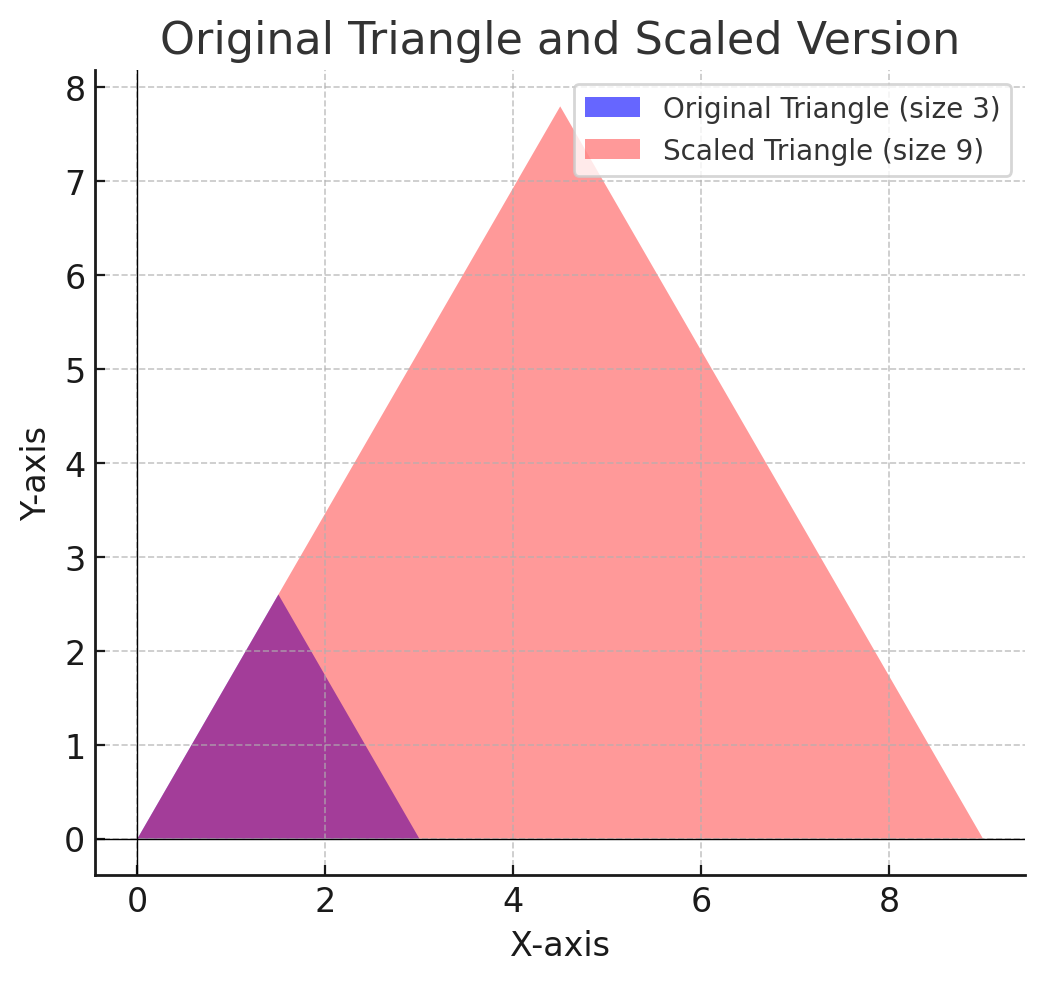
\includegraphics[width=0.4\textwidth]{similar_triangle.png} % Replace with your image path
        \caption{A triangle of size 3 and its scaled version by a factor of 3}
    \end{figure}
\end{frame}



\begin{frame}{Similar Triangles Postulates}
    \begin{itemize}
        \item \textbf{Angle-Angle (AA) Similarity Postulate:} 
        \begin{itemize}
            \item If two angles of one triangle are congruent to two angles of another triangle, the triangles are similar.
        \end{itemize}

        \item \textbf{Side-Angle-Side (SAS) Similarity Postulate:} 
        \begin{itemize}
            \item If one angle of a triangle is congruent to one angle of another triangle, and the sides that include these angles are proportional, then the triangles are similar.
        \end{itemize}

        \item \textbf{Side-Side-Side (SSS) Similarity Postulate:} 
        \begin{itemize}
            \item If the three sides of one triangle are proportional to the three corresponding sides of another triangle, the triangles are similar.
        \end{itemize}
    \end{itemize}
    
\end{frame}

\begin{frame}
    \frametitle{Parallel Lines}
    
    \begin{itemize}
        \item \textbf{Definition:} Two or more lines that are always the same distance apart and never meet, no matter how far they are extended.
        \item They run in the same direction and have the same slope.
        \item Example: Think of train tracks running side by side—they never cross each other.
    \end{itemize}
    
    \begin{center}
        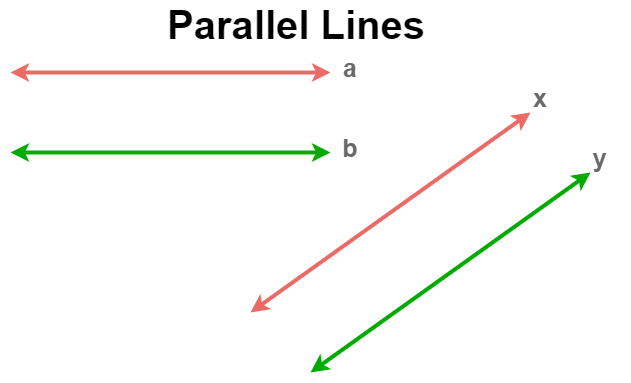
\includegraphics[width=0.5\textwidth]{Parallellines.png} % Add an appropriate image to illustrate parallel lines
    \end{center}

\end{frame}


\begin{frame}
    \frametitle{Transversals}
\end{frame}


% % \begin{frame}
% % \frametitle{What is a Unit Circle}
% % \begin{block}{The Unit circle}
% %     The unit circle is the circle with radius 1 centered at the origin 
% % \end{block}
% % \begin{block}{Equation of unit Circle}
% %     The unit circle in the xy-plane is the set of points (x,y) such that
% %     $$x^{2} + y^{2} = 1$$
    
% % \end{block}

% % \end{frame}

% % \begin{frame}
% %     \frametitle{Radius corresponding to a positive angle}
% %     \centering
% %     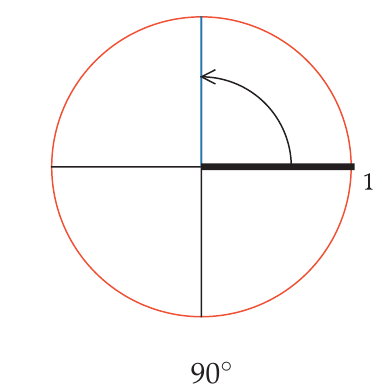
\includegraphics[scale=0.5]{1.png}

% % \end{frame}

% % \begin{frame}
% %     \frametitle{Radius corresponding to a negative angle}
% %     \centering
% %     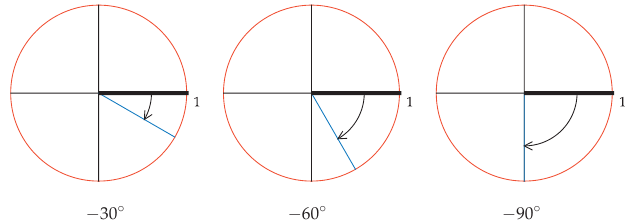
\includegraphics[scale=0.5]{2.png}

% % \end{frame}

% % \begin{frame}
% %     \begin{block}{Positive and Negative Angles}
% %         \begin{itemize}
% %             \item Angle measurements for a radius on the unit circle are made from the
% %             positive horizontal axis.
% %             \item Positive angles correspond to moving counterclockwise from the positive
% %             horizontal axis.
% %             \item Negative angles correspond to moving clockwise from the positive hori-
% %             zontal axis.
% %         \end{itemize}
% %     \end{block}
% % \end{frame}

% % \begin{frame}
% %     \begin{figure}[h]    
% %         \begin{minipage}[b]{0.3\textwidth}
% %         \centering
% %         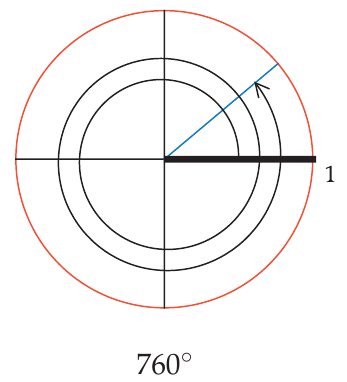
\includegraphics[scale=0.25]{3.png}
% %         \caption{+ve angle}
% %     \end{minipage}
% %     \begin{minipage}[b]{0.3\textwidth}
% %         \centering
% %         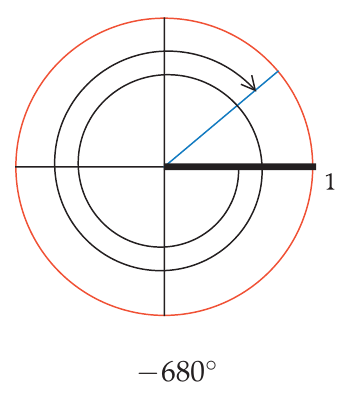
\includegraphics[scale=0.25]{4.png}
% %         \caption{-ve angle}
% %     \end{minipage}
% % \end{figure}
% % \begin{block}{cyclic hehaviour of angles}
% %     A radius of the unit circle corresponding to $\theta$ degrees also corresponds to
% % $\theta + 360n$ degrees for every integer n.
% % \end{block}
% % \end{frame}


% % \begin{frame}
% %     \frametitle{Length of a Circular Arc}
% %     \centering
% %     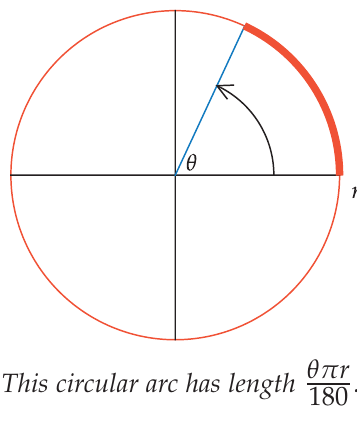
\includegraphics[scale=0.5]{5.png}
% % \end{frame}

% % \begin{frame}
% %     \frametitle{Radians}
% %    \begin{block}{Radians}
% %     Radians are a unit of measurement for angles such that $2\pi$ radians correspond
% %     to a rotation through an entire circle.
% %    \end{block}
% % \end{frame}

% % \begin{frame}
% %     \frametitle{Radians}
% %     \centering
% %     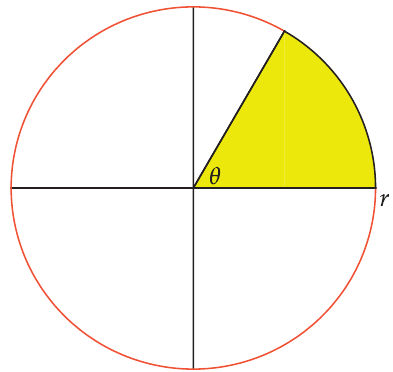
\includegraphics[scale=0.3]{6.png}
% % \end{frame}
% % \begin{frame}
% %     \frametitle{Radians}
% %    \begin{block}{Degree to Radians}

%     $$ 360^{\circ} = 2 \pi radians $$
%     $$ 1 ^{\circ}  = \frac{2 \pi}{360} radians $$
    
%    \end{block}
% \end{frame}

% \begin{frame}
%     \frametitle{Arc Length}
%     \begin{block}{length of a circular arc}
%         If $0 < \theta \leq 2\pi$ , then a circular arc on the unit circle corresponding to $\theta$ radians
%         has length $\theta$         
%     \end{block}
% \end{frame}

% \begin{frame}
%         \begin{figure}[h]    
%             \begin{minipage}[b]{0.3\textwidth}
%             \centering
%             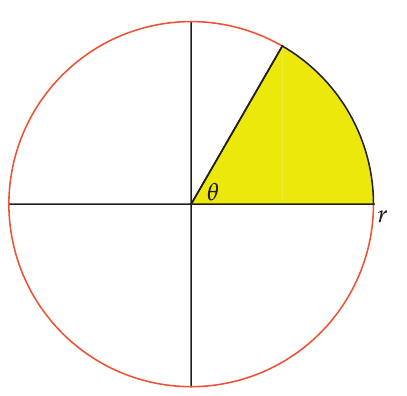
\includegraphics[scale=0.25]{7.png}
%             \caption{Area of slice}
%         \end{minipage}
%     \end{figure}
%     \begin{block}{Area of slice}
%         A slice with angle $\theta$ radians inside a circle with radius $r$ has area $\frac{1}{2} \theta r^{2}$ .
%     \end{block}
% \end{frame}

% \begin{frame}
%     \frametitle{Cosine and Sine}
%     \begin{figure}[h]    
%         \begin{minipage}[b]{0.8\textwidth}
%         \centering
%         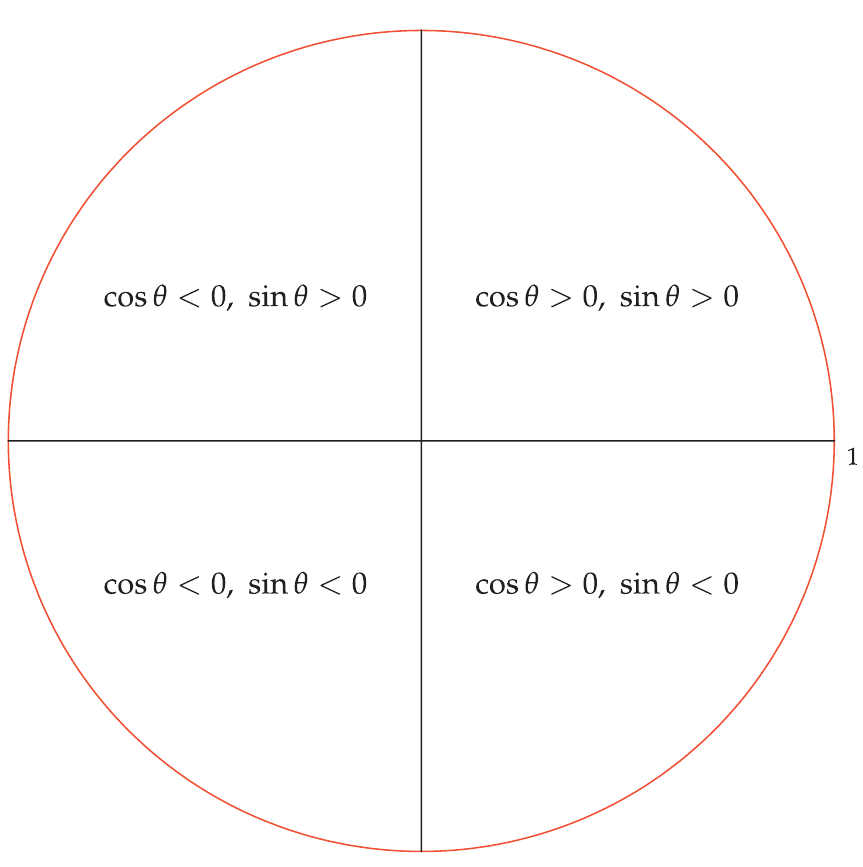
\includegraphics[scale=0.22]{8.png}
%         \caption{sin and cos}
%     \end{minipage}
% \end{figure}
% \end{frame}
 \end{document}